\documentclass[a4paper,12pt]{article}

\usepackage{etoolbox}
\usepackage{fancyvrb}
\usepackage[T1]{fontenc}
\usepackage{graphicx}
\usepackage{import}
\usepackage{listings}
\usepackage{minted}
\usepackage{caption}
\usepackage{url}
\usepackage{courier}

\usepackage[
	% Prevent hyperlinks from getting an ugly border
    hidelinks,
    % Set proper PDF metadata
    pdftex,
    pdfauthor={Dennis Fischer},
    pdftitle={Detecting Process Memory Tampering},
    pdfsubject={TBD},
    pdfkeywords={dll injection, code injection, injection, code cave, nop, nop hopping, memory, tampering, detection, dll}
]{hyperref}
\usepackage{sections/_meta/tumlogo}

% Don't display "References" when rendering the bibliography
\patchcmd{\thebibliography}{\section*{\refname}}{}{}{}

% Use appropriate font size for line numbers in listings
\renewcommand{\theFancyVerbLine}{{\small\arabic{FancyVerbLine}}}
\lstset{basicstyle=\ttfamily}

\newcommand{\codefile}[2]{
\inputminted[breakanywhere, breaklines,fontsize=\scriptsize, frame=single, mathescape, linenos, numbersep=5pt, numbersep=5pt, xleftmargin=0pt]{c}{SourceCode/\detokenize{#1#2}}
\captionof{listing}{Code from \detokenize{#2}}
\label{code:\detokenize{#2}}
}

\newcommand{\syscall}[1]{\texttt{#1}}


\setlength{\footnotesep}{0.4cm}
\setlength{\skip\footins}{0.5cm}

\def\doctype{Bachelor's Thesis in Informatics}
\def\title{Detecting Process Memory Tampering}
\def\germantitle{Erkennen von Prozess Speichermanipluationen}
\def\author{Dennis Fischer}
\def\date{Februar 15, 2016}


\begin{document}
\sloppy
\thispagestyle{empty}

\def\bcorcor{0.15cm}
\addtolength{\hoffset}{\bcorcor}

\thispagestyle{empty}

\vspace{4cm}

\begin{center}
  \oTUM{4cm}
  
  \vspace{5mm}
  
  \huge DEPARTMENT OF INFORMATICS\\
  
  \vspace{0.5cm}
  
  \large TECHNISCHE UNIVERSIT{\"A}T M{\"U}NCHEN\\
  
  \vspace{1mm}
\end{center}

\vspace{15mm}

\begin{center}
  {\Large \doctype}

  \vspace{20mm}

  \setlength\lineskip{8pt}
  {\LARGE \bf \title}\\%[3ex]

  \vspace{15mm}

  {\LARGE \author}

  \vspace{10mm}

  \begin{figure}[h!]
    \centering
    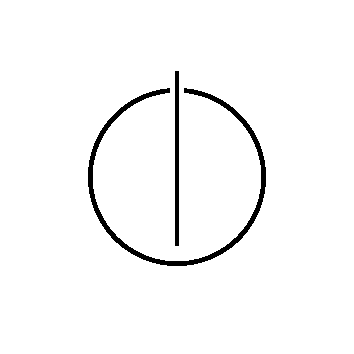
\includegraphics[width=4cm]{sections/_meta/informat.png}
  \end{figure}
\end{center}

\thispagestyle{empty}

\def\bcorcor{0.15cm}
\addtolength{\hoffset}{\bcorcor}

\thispagestyle{empty}

\vspace{4cm}

\begin{center}
  \oTUM{4cm}
  
  \vspace{5mm}
  
  \huge DEPARTMENT OF INFORMATICS\\
  
  \vspace{0.5cm}
  
  \large TECHNISCHE UNIVERSIT{\"A}T M{\"U}NCHEN\\
  
  \vspace{1mm}
\end{center}

\vspace{15mm}

\begin{center}
  {\Large \doctype}

  \vspace{20mm}

  \setlength\lineskip{8pt}
  {\LARGE \bf \title}\\%[3ex]

  \vspace{10mm}

  {\LARGE \germantitle}
\end{center}

\vfill

\renewcommand{\arraystretch}{0.7}

\begin{center}
\begin{tabular}{l@{\hskip 1cm}l}
  {\Large \bf Author:} & {\Large Dennis~Fischer} \\\\
  {\Large \bf Supervisor:} & {\Large Prof.~Dr.~Alexander~Pretschner} \\\\
  {\Large \bf Advisor:} & {\Large M.Sc.~Sebastian Banescu} \\\\
  {\Large \bf Submission date:} & {\Large 15.~Februar~2016}
\end{tabular}
\end{center}

\thispagestyle{empty}

\vspace*{\fill}
\begin{flushright}
\noindent \textit{I confirm that this bachelor's thesis is my own work \\ and I have documented all sources and material used.\\[\baselineskip]}
M{\"u}nchen, 15. Februar 2016 \\[3.5\baselineskip]
\underline{\hspace{6.5cm}}
\end{flushright}


\newpage
\thispagestyle{empty}
\null

% \newpage
\thispagestyle{empty}
\section*{Abstract}

TBD

\newpage
\pagestyle{empty}
\tableofcontents

\newpage
\pagestyle{plain}
\setcounter{page}{1}

% PUT Content here!
\section{Introduction}
\label{chap_introduction}
\subsection{Motivation}
\gls{PMT} describes the process of unwanted memory modifications of another process. These modifications can lead to unwanted behavior of the target application, resulting in several different security flaws like integrity, availability and confidentiality. The first, integrity, might no longer exist, as the intended behavior of the application is changed. Often applications are modified in such a way, that it is not possible to guarantee unchanged behavior. The second, availability, can no longer be ensured if the changes lead to longer runtimes. This results in a higher memory and CPU usage and the machines limit are reached sooner than expected, leading to unexpected crashes or in general, service outages. The last, confidentiality is broken, because the attacker can access the process' memory, thus allowing the attacker to read sensitive information like passwords or shared keys, and execution of injected code, altering the programs behavior. \gls{PMT} is present on every operating system and can be applied to any application running on the OS, with typical examples being \emph{games}. \gls{PMT} can be used to modify the games behavior, which is referred to as cheating, because the user gets an unfair advantage against other users.
\subsection{Problem}
"A browser hijacker is software that modifies the default browser behaviour" \cite{automatedspywarecollection}. That is a  vague definition but reflects one possible candidate of \gls{PMT} attacks. As a browser is required to view websites, it is used by over three billion \cite{cia} different users, making it a valuable attack target. An attack is able to change default settings like the search engine, which then gain the attacker additional ad revenues from more visitors. Traffic redirection proves to be very simple with \gls{PMT} and thus allows to make phishing activities look harmless, as they can no longer be distinguished from the original website.
In games, especially in online games that are based on a large amount of user-inputs, \gls{PMT} can be applied to create powerful cheats that are hard to detect. The cheater hereby has to reverse engineer the game once to receive a table of offsets. This table of offsets contains the relative memory locations, the relative addresses, that can be used to access important game information. In cheat forums, such a table is typicially represented in text format with key-value pairs \cite{offsets}. By directly changing the data of the game, \emph{aimbots}, \emph{wallhacks} and \emph{scripts} can be created easily. The unfair advantage gained by the cheat destroys the games audiences fun and in the long term significantly reduces the number of active players. Nevertheless cheats are used knowing these consequences, as the short term fun is more pleasant for the cheater. \gls{PMT} detection is a crucially important thing in online games like First Person Shooters, as the whole game play relies on user input, but often is very hard to achieve to due lack of knowledge and legal issues. Legal issues exist during the deployment of the users software, because an anti cheat application usually requires root access to detect cheats. However, this stands in contrast to data protection laws, which deny such deep access without the users permissions. The game developers then need to make a legal contract with the user, often defined within the \gls{EULA} or Terms of Service. Root access raises another problem, as the users might not trust the anti cheat developers because of pasts incidents. One example in the First Person Shooter area is the game \emph{Counterstrike: Global Offensive}, which is, according to the active players and viewers, the third most played e-Sports game. As such, several leagues exist which often ship their own anti cheat system. The \gls{ESEA}, a counterstrike league, was fined one million us-dollar by the US Superior Court of California, County of San Francisco \cite{esea} in case \emph{CGC-13-532593}, for secretly mining bitcoins in their anti cheat. 
\subsection{Goal}
The goal of this thesis is to create a software that detects and if possible prevents \gls{PMT} attacks on \emph{Google Chrome}, so that it can no longer be hijacked via \gls{PMT}.
\subsection{Contribution}
Current attacks and their associated defenses are evaluated against PMT and ideas for new defenses are researched and developed.
\subsection{Outline}
In chapter \ref{chap_background} current attacks and defenses for PMT are explored. Afterwards in chapter \ref{chap_implementation} new defenses are designed and evaluated for their performance and security in chapter \ref{chap_evaluation}. Finally in chapter \ref{chap_futurework} future work is presented.
\section{Background}
\label{sec:background}
To get a better understanding and an overview of the thesis goal, the following chapter will deal with windows internal concepts, existing attacks and their existing countermeasures.
\subsection{Windows important Concepts}
\subsection{Attacks}
\subsubsection{\emph{Registry} based injection}
\emph{Registry} based injection uses a special \emph{Registry} key\footnote{The \emph{Registry} key can be found at \syscall{HKEY\_LOCAL\_MACHINE\textbackslash Software\textbackslash Microsoft\textbackslash\allowbreak Windows NT\textbackslash CurrentVersion\textbackslash Windows}} that can be used to inject \gls{DLL} files into almost any process. For that reason the shown attack tree in Figure~\ref{fig:attacks_external} lists this technique under the group of \gls{DLL} injections in node [1.2.1]. \glspl{DLL} can be added by writing the full path to the file into this \emph{Registry} key, with multiple paths separated by semicolons. To make this injection technique work, two conditions have to apply:
\begin{enumerate}
\item The \gls{DLL} file is having a security descriptor that allows execution. Otherwise the \gls{DLL} will not get loaded into the target process.
\item The \gls{MSDN} \cite{msdn_appinitdlls} lists the usage of \syscall{User32\allowbreak.dll} in the target process as a requirement or otherwise the \glspl{DLL} listed in the \emph{Registry} will not get loaded.
\end{enumerate}
However, these two conditions are easy to fulfill. The first condition is by default true, because the default security descriptor on \gls{DLL} files allow execution. Active interaction by other programs or the user is required to change the security descriptor. The second condition is most of the time fulfilled. \syscall{User32.dll} is used in almost every process and in general it can be assumed that the \gls{MSDN} requirement is fulfilled. To make this attack work, a second \emph{Registry} key, \syscall{LoadAppInit\_DLLs}, has to be changed to value 1, in order to activate this \emph{Registry} based injection. By default this value is set to 0 and cannot be changed without admin privileges.
Defending against this kind of attack is comparably easy, by checking \syscall{AppInit\_DLLs} value and enumerating all loaded modules (\glspl{DLL}). If a match is found and considered to be unwanted, it can be unloaded or as a safety measurement the application is terminated. As for \emph{Google Chrome}, there is no validation currently in place and \emph{Registry} based injection can be used to load arbitrary \gls{DLL} files.
\subsubsection{\syscall{SetWindowsHookEx} Injection}
Another way besides \emph{Registry} based injections is using the \syscall{SetWindowsHookEx} function of the \emph{Windows} \gls{API} to inject a \gls{DLL} file. It requires no special privileges to be executed and can be used to  hook into a specific application or being system wide. A hook in this context is a callback function that gets executed whenever a certain event is occurring. In terms of \syscall{SetWindowsHookEx}, there are according to the \gls{MSDN} \cite{msdn_setwindowshookex} 15 different possible types of events that can be registered for, of which some can only be system wide. The hook procedure that is required as parameter for \syscall{SetWindowsHookEx} has to be located in a \gls{DLL} file. The \gls{DLL} to be injected is loaded by the operating system into the current process, to make the specified callback function available. An example code is shown in Appendix~\ref{appendix:setwindowshookex}. As this attack is also a based on \gls{DLL} injections the attack tree of Figure~\ref{fig:attacks_external} lists this attack under [1.2.2] in external modifications. 

\medskip

The \gls{DLL} will not get loaded into the target process until the event is triggered and the registered hook is called for the first time. The callback procedure gives different opportunities to make use of this created situation. An additional thread can be started from the callback procedure or the called driver entry function to make the injection independent of the hook callback function. As this module and especially any created thread are running in the context of the remote process, the \gls{DLL} code has full access to the process' memory. Internal memory modifications can be performed, which will get explained in Section \ref{sec:internal_modifications}. As well as for \emph{Registry} based injections, \emph{Google Chrome} does not prevent \syscall{SetWindowsHookEx} \gls{DLL} injections.
\subsubsection{DLL Replacement}
The last missing DLL injection technique of the given attack tree in Figure \ref{fig:attacks_external} is DLL Replacement. The idea is to replace an existing DLL file with a patched or completely different DLL, which is possible due to the windows internal concepts. Every DLL exports functions that can be called from a program. The attack know creates a new DLL file, that exports the same functions and internally redirects all calls to the original DLL file. Therefore the functionality of the application stays the same and the attack is harder to detect. It is now possible to use on of the exported functions to execute other, new code that performs malicious activities.

\subsubsection{\syscall{WriteProcessMemory} external modifications}
\syscall{WriteProcessMemory} is just like the previously discussed \syscall{SetWindowsHookEx} a function available through the Windows API. This function allows to write into the virtual memory of a target process and allows modifying existing data or code. There are several ways to make use of this function, one of them being DLL injection with the \syscall{CreateRemoteThread} and \syscall{LoadLibrary} functions. 

\paragraph{\syscall{CreateRemoteThread} DLL Injection}
DLLs can be loaded into a target process by loading its path into the target memory with \syscall{WriteProcessMemory} and creating a new thread via \syscall{CreateRemoteThread} that calls \syscall{LoadLibrary}. This kind of attack can be used on any process running under the same integrity level and therefore is very widely used in game cheating. At first, a handle to the target process is requested via \syscall{OpenProcess} with \syscall{PROCESS\_VM\_WRITE} and \syscall{PROCESS\_VM\_OPERATION} access rights, which are required to execute the important \syscall{WriteProcessMemory} function. If the permissions are missing, \syscall{WriteProcessMemory} is not able to modify the virtual memory of the target process. Virtual memory protection flags don't have to be changed manually, as this is already happening inside \syscall{WriteProcessMemory}. After that, a large enough amount of memory is allocated inside the target process with \syscall{VirtualAllocEx}, to hold the full path of the DLL. Next \syscall{WriteProcessMemory} is used to transfer the DLL path into the target memory space and finally the injection can be completed by calling \syscall{CreateRemoteThread}, which finally loads the DLL with the \syscall{LoadLibrary} function. The allocated memory segment is used as a parameter for the \syscall{LoadLibrary} function call. With the now loaded DLL, arbitrary code can get executed by the DLL, either via using \syscall{CreateRemoteThread} again or via the DLLs entry point.
An example of a very basic DLL injection using \syscall{WriteProcessMemory} and \syscall{CreateRemoteThread} can be found in appendix \ref{appendix:writeprocessmemory}. Again, chrome shows no existing defense mechanisms against direct memory modification.

A second way to make use of \syscall{WriteProcessMemory} is modifying the targets code inside memory, to execute different instructions than intended. This technique is also commonly known as function hooking or function detouring, which is described in the next paragraph. 
\paragraph{Function detouring}
\input{sections/background/attacks/fig_detours}
Function detouring has been greatly simplified by the Detours\cite{msdetours} library of Microsoft, but can also be achieved by memory modification with \syscall{WriteProcessMemory} or assembly code. Figure \ref{fig:detours} shows the difference between a function before and after detouring. The function call at the top shows a invocation without interception. The source function calls the target function without any indirection and after the code of the target function has been executed, returns to the calling source function. Detouring makes use of this structure by placing a detour and a trampoline function in between these calls. The source function will now use an indirect call to the target function, by first calling the detour part, which gives space to execute arbitrary code. To do that, a \syscall{jmp} instruction is placed at the beginning, and the original instructions are saved and copied to the trampoline function. After that, the detour function continues with the trampoline function, which executes the copied instructions and ensures that the target function works as if there was no detour placed. Finally, the whole function stack will return, this time skipping the trampoline function, as it was just used to hold the copied instructions. 

A detection of this technique is very difficult and can only be obtained by measuring the performance of called functions. If execution then takes in average exceptionally longer, there might be a detoured function. It is however impossible to make this detection reliable for all functions, as the systems unexpectable scheduling and load influence the resulting performance.

\subsubsection{Buffer overflows}
Buffer overflows are among the most severe security problems of modern applications, as they are hard to detect, and are introduced by simple programming errors that weren't previously found in testing and quality assurance steps. Even though they are hard to find, once used they allow the attacker to hopefully execute arbitrary code. If code execution is not possible, sensitive information might get revealed. One of the most severe examples of the past was the so called "Heathbleed bug", which affected millions of servers worldwide, as it was present in the much used OpenSSL library. Even though the attacker couldn't execute code, he was able to get sensitive information about the SSL certificates private key and thus break any security put in place by the SSL protocol. This attack is the last one of Figure \ref{fig:attacks_external} and also a external modification. In contrast to the other previously shown attacks there are several countermeasures existing to mitigate the resulting exploit, which will be discussed in chapter \ref{sec:defenses}.

\subsubsection{Internal modifications}
\label{sec:internal_modifications}
\begin{figure}[h]
\centering
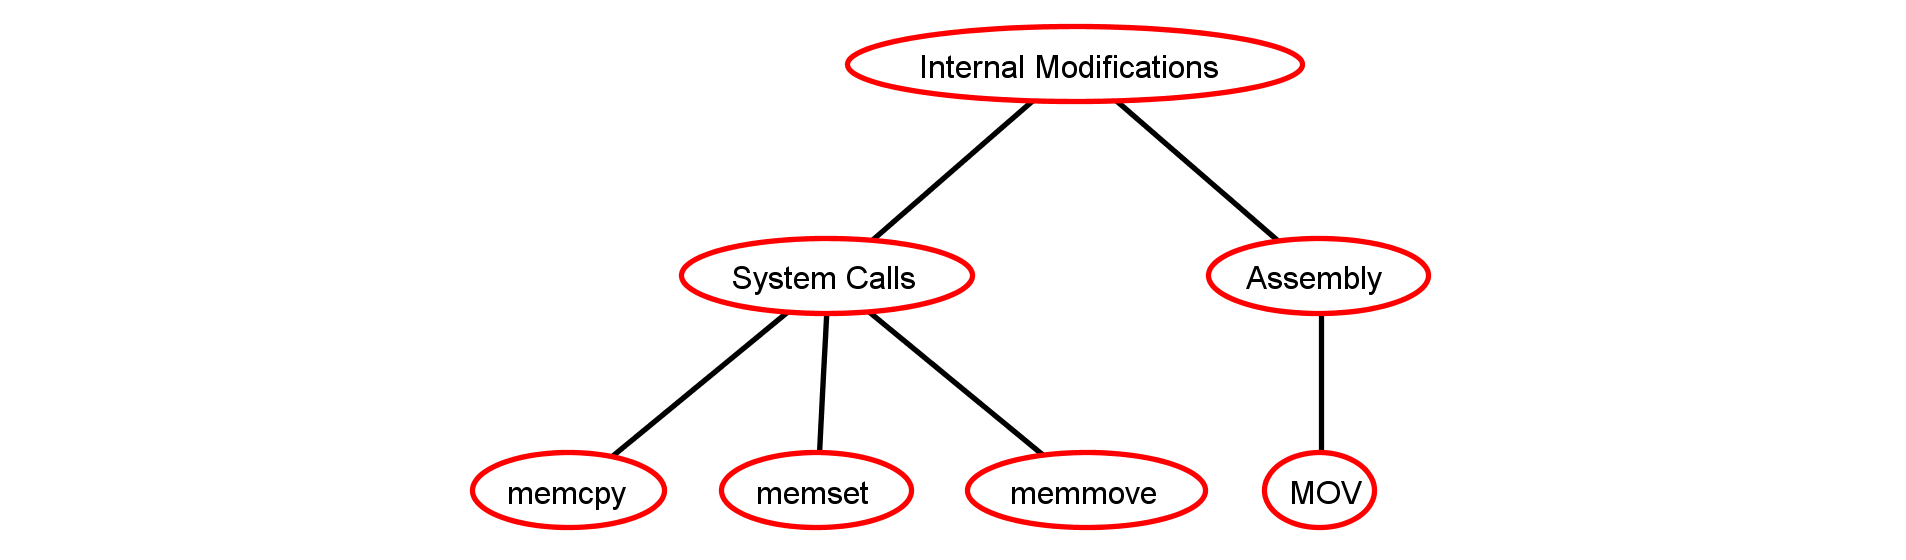
\includegraphics[scale=0.45]{sections/adtrees/InternalModificationsWithoutDefenses.png}
\caption{This attack tree shows possible attacks that are grouped under internal modification.}
\label{fig:attacks_internal}
\end{figure}
A group of attack is internal modifications which is in contrast to external modifications occurring from inside the process virtual memory. As the attacker is already inside the virtual memory, modification is easier and less restricted then the previously shown external modifications. The attacker can make use of existing functions like \syscall{memcpy} or \syscall{memset}, to modifiy the values inside memory, without having to use the indirection via \syscall{WriteProcessMemory}. Besides the present \syscall{mem*} functions, the attacker can also make use of assembly code. Figure \ref{fig:attacks_internal} shows this type of attack. The assembly part outlines the \syscall{mov} instruction, as it is mainly used to detour functions without the usage of exported API functions.
The shown attacks are represented in figure \ref{fig_attacks} in an attack tree.
\begin{figure}[!h]
	\centering
	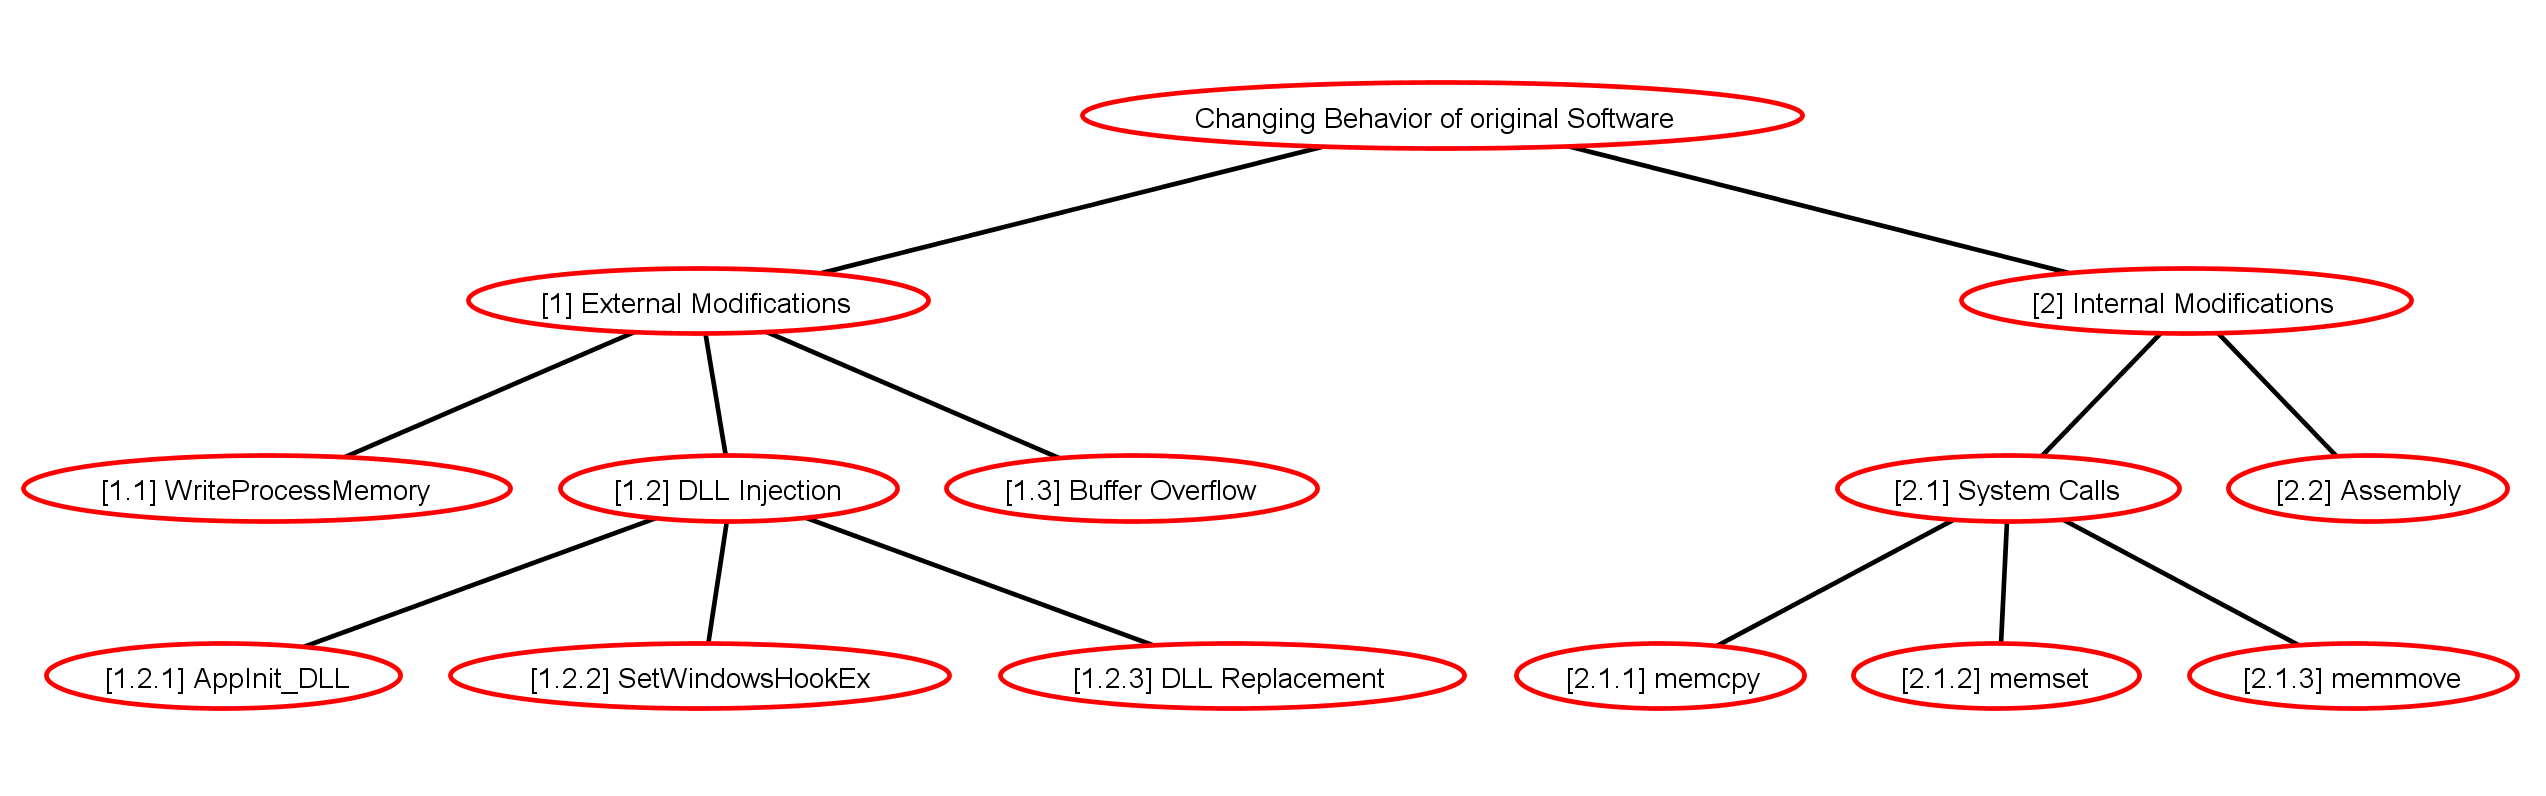
\includegraphics[angle=90,height=\textheight,keepaspectratio]{sections/adtrees/ProcessVirtualMemoryWithoutDefenses.png}
	\caption{An attack tree combining all of the shown attacks}
	\label{fig:attacks}
\end{figure}

\subsection{Defenses}
\label{sec:defenses}
This section describes existing defenses against the outlined attacks of Section \ref{sec:attacks}.
\subsubsection{Adress Space Layout Randomization}
\subsubsection{Data Execution Prevention}
\label{sec:dep}
The second existing defense prevents code execution from data memory pages by setting a special \syscall{No Execute bit} \cite{msdn_dep} in hardware onto the memory page. This protection is done by default for every started process. A process will allocate a certain number of memory pages, of which one part is used for the code, and the other for the data. The data sections will automatically get assigned the \syscall{NX bit} and the code pages will not. The attacker might be able to inject code into the data region, but if the application tries to execute the injected code, it is not possible due to the \syscall{NX bit} and an exception is raised leading to an application crash. Thus the attack is prevented and especially buffer overflows can no longer get exploited.

However, for the other attacks based on \syscall{WriteProcessMemory} or \gls{DLL} injection, this defense mechanism serves no purpose. The attacker can use the \emph{Windows} \gls{API} method \syscall{VirtualProtect} \cite{msdn_virtualprotect} to unset the \syscall{NX bit} of data pages and therefore also make use of them for code injection. Additionally, this change might not even be needed. The attacker could do the code injection in a three step manner: 
\begin{enumerate}
\item Code is injected into the \emph{code region} of the process. As the main purpose of this code is removing the \syscall{NX bit} of data pages, the resulting code can be much smaller compared to the actual exploit that should be executed.
\item Code is injected into the \emph{data region} of the process. This is the actual exploit that should run.
\item The injected code of Step 1 will get executed by random or can actively be started from outside. The \syscall{NX bit} gets unset and the injected exploit of Step 2 is now executable. The exploit of Step 2 can now be started to complete the attack.
\end{enumerate}
\subsubsection{Mandatory Integrity Control}
\begin{figure}[h]
\centering
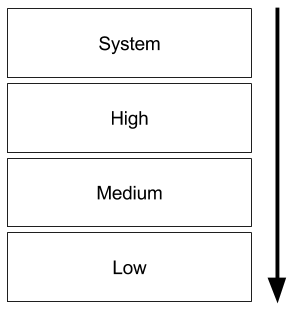
\includegraphics[scale=0.5]{sections/background/defenses/mic.png}
\caption{The hierarchy of integrity levels with decreasing permissions from top to bottom}
\label{fig:mic}
\end{figure}
Mandatory Integrity Control is based on the Bell-LaPadula \cite{eckert2014sicherheit} model and multi level security. On Windows systems, there are four different integrity levels with decreasing privileges: System, High, Medium and Low. Figure \ref{fig:mic} shows an example of the integrity hierarchy, sorted form top to bottom by decreasing permissions. By definition it is not possible to access an object of higher integrity level than the accessing object. Therefore, if process memory tampering is used, both processes need to have at least the same integrity level. The fourth integrity level \syscall{System} cannot be reached from the logged in user. Processes can now be started with one of the remaining integrity levels. By default, all processes receive \syscall{Medium} integrity level. \syscall{Low} needs to be explicitly assigned and \syscall{High} is used only if the process is started with elevated permissions. Thus, as most processes run with \syscall{Medium} integrity level, mandatory integrity control is useless in preventing memory tampering. Even if chrome will receive \syscall{High} integrity level, this cannot be recommended as chrome is not trustworthy. If an attack is successful, the attacker will now have more access right than with the default \syscall{Medium} integrity level.
\section{Design and Implementation}
The upcoming Design and Implementation chapter describes possible countermeasures to the previously shown attacks. The best working one is then being implemented.
\subsection{Requirements}
\subsection{Design and Architecture}
The attacks of Section \ref{sec:attacks} can be classified into two groups which have to be handled separately in order to increase security on the target platform. Attacks to the process virtual memory that have to use \gls{WPM}, which form the first group and attacks that are relying on a \gls{DLL} load during their initialization to execute their malicious code from inside, which form the second group. This classification makes it possible to design effective countermeasures that can not be avoided by attacks.

\begin{figure}[!htbp]
\centering
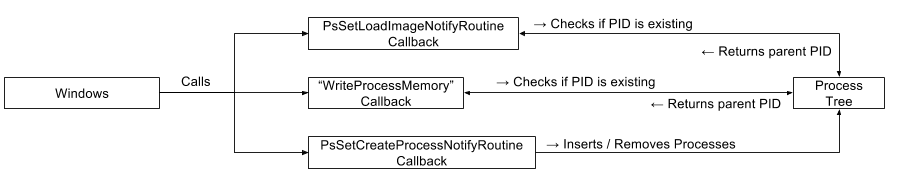
\includegraphics[angle=90,scale=0.6]{sections/implementation/interaction.png}
\caption{The interaction of the drivers components}
\label{fig:interaction}
\end{figure}

The classification into the two groups, \gls{DLL} and \gls{WPM}, is used to for the architecture design. Figure \ref{fig:interaction} shows the interacting components in an abstract representation. \emph{Windows} offers three entry points that will get called by the kernel, whenever a process is started, opened or a \gls{DLL} is loaded. The registered callback functions will then need to do several checks on the given information and based on this allow or deny execution.  
\paragraph{Process Tree Structure}
The \syscall{PsSetCreateProcessNotifyRoutine} callback function is called whenever a process is created or destroyed. Accordingly, whenever this callback function is executed, the process is inserted into the process tree structure on process creation, and removed from the process tree structure on process deletion. The process tree hereby maintains a list of lists, which is shown in Figure \ref{fig:listoflists}.
\begin{figure}[!htbp]
\centering
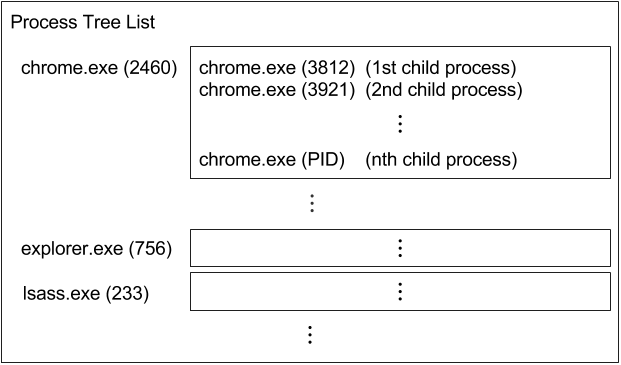
\includegraphics[scale=0.6]{sections/implementation/listoflists.png}
\caption{The process tree structure. A list of parent processes with their children}
\label{fig:listoflists}
\end{figure}
Each list separates the processes parents with their children from other processes. If the process tree gets queried for a specific \gls{PID} the parent \gls{PID} gets returned. To illustrate this interaction, the data of Figure \ref{fig:listoflists} is used for an example. If the process tree is queried with \gls{PID} 3812, a lookup in the process tree occurs to find a process with \gls{PID} 3812. In this case, the process is a child of chrome.exe with \gls{PID} 2460.
Because process 3812 is a child process, its parent 2460 is returned. For a second example, consider the process tree being queried for \gls{PID} 2460. Another lookup is done and a process with \gls{PID} 2460 is found. Because 2460 is a parent process, the process tree structure returns the value 2460.

\paragraph{DLL Component}
The last callback function of Figure \ref{fig:interaction}, \syscall{PsSetLoadImageNotifyRoutine}, is called by the \emph{Windows} kernel whenever a DLL is loaded. The callback routine queries the process tree structure for a given \gls{PID} to see if this is a chrome.exe process. If it is a chrome.exe process, the callback generates a hash of the DLL file, compares it to a whitelist and if a match can not be found takes action to prevent DLL loading.

\paragraph{WPM Component}
To prevent the group of \gls{WPM} attacks, a WPM callback is registered which checks if the given \gls{PID} is in a whitelist. If it is not, the request is denied by removing the required permissions to execute \gls{WPM} attacks. Because \glspl{PID} are dynamically assigned by the kernel and the possibility of reusing \glspl{PID}, a internal structure, a process tree, needs to be maintained. This thus adds communication between the three callback functions and the process tree as seen in Figure \ref{fig:interaction}.
\subsection{Implementation}
\label{sec:implementation} 

\subsection{Blocking \syscall{WriteProcessMemory} with a kernel mode driver}
The newly created problem with the modified \gls{ACL} can be solved by creating a driver running in kernel-mode. As reading memory, checking files and running processes are a common problem when writing anti virus software, Microsoft introduced object manager routines since Windows Vista to provide an efficient way of reacting onto these events. A driver will then use \syscall{ObRegisterCallbacks} to get notified whenever processes are created, files are opened and images (\glspl{DLL} and EXEs) are loaded. This functionality offers the programmer to create a pre- and post-execution callback function, that gets called whenever a process tries to receive a process handle. Microsoft offers an example driver using \syscall{ObRegisterCallbacks} at \cite{github_obcallback} and shows how to modify the requested process handle permissions to prevent termination by other applications such as the task manager. 

In order to protect chrome, the same actions described earlier will now be taken from inside the driver. Newly created process handles will be restricted to non virtual memory modifying permissions and the existing problem with inter process communication can be resolved by not restricting chromes child processes explicitly and giving them a full access handle. Appendix \ref{appendix:driver} shows an implemented driver to fulfill the requirements.

However, a naive implementation that just checks for process' executable file name may result in an access gain for the attacker. The injecting process simply has to be named chrome.exe and can gain access to the original chrome.exe. In this case, the implementation restricts outside access regardless of the given process name successfully. Children and parent \glspl{PID} are stored inside two separate tables that are on access checked if they contain target and source process ids. The driver is using a dynamic list structure, so that an unlimited number of processes can be tracked. Finally the check for access rights can be done by finding a given \gls{PID} inside the defined lists and returning a hash value, which uniquely identifies the process. 

A good hash for this tree is the parent \gls{PID}, as the process hierarchy is tracked inside the list. Only if both find operations result in a match of the returned \glspl{PID}, access is granted and no restriction is applied. Entries of the list (parent or child process) will get removed as soon as they exit, so that the remaining list is kept clean from garbage and reassignments of the same \gls{PID} do not lead to a security hole.

\subsection{Blocking DLL Injection with a kernel mode driver}
As previously stated, the resulting implementation already uses a kernel mode driver to prevent \gls{WPM} calls. It is therefore a suitable start point to prevent \gls{DLL} injections without being required to hook into the kernel. The Windows \gls{API} for drivers offers the \syscall{PsSetLoadImageNotfiyRoutine} function call, to register a callback function that is executed whenever a \gls{DLL} is mapped into memory. During the function call, the process is in a suspended state and thus execution of the \gls{DLL} has not begun. However, this entry point for \gls{DLL} load prevention is not optimal, as this function call occurs after the \gls{DLL} was already mapped into memory and a pre loading callback would be better to use in this situation. Unfortunately, this callback function does not exist so far, so the implementation has to rely on the post load callback.

To make use of \syscall{PsSetLoadImageNotifyRoutine}, the \gls{IRQL} may not be changed, because otherwise it can lead to a deadlock or even make the system crash in a blue screen of death. Most notably is the fact that the function call occurs on \gls{IRQL} \syscall{PASSIVE\_LEVEL} and special kernel mode \glspl{APC} are disabled. This is at first a major limitation to naive implementations. Opening and reading file calls will not complete, as the underlying \gls{APC} event is not sent, thus in a naive implementation, reading a file seems impossible at a first glance. The reason for the disabled special kernel mode \glspl{APC} is a previous call to the \syscall{KeEnterGuardedRegion} function, so a call to \syscall{KeLeaveGuardedRegion} can enable \gls{APC} events again. However, this should not be done here, as the result turns out to be unpredictable and leading to random deadlocks or failing accesses on files.

Having a deeper look at the windows kernel with a kernel debugger, a solution can be obtained by using a second running thread, a so called work item, which execution is handled separately by the system. The advantage of this are the enabled special kernel mode \glspl{APC} and the possibility to freely change the \gls{IRQL} during execution. One major disadvantage of this way is, that some sort of thread synchronization between the work item and the initial callback function has to be introduced and thus resulting into driver typical busy waiting, which is still faster than non busy waiting and eventually occurring context changes. 

A file handle can now be obtained and from the file data a sha256 \cite{eckert2014sicherheit} hash is generated, which is used later to compare it to a known whitelist of \gls{DLL} files. The Windows \gls{API} offers several different ways of obtaining a valid file handle with functions like \syscall{ZwOpenFile} or \syscall{ObOpenObjectByPointer}. The second function \syscall{ObOpenObjectByPointer} will generate a handle from a given pointer to an object. That is exactly what can be found inside the input parameters of the \syscall{PsSetLoadImageNotifyRoutine} callback. The image info can be extended to obtain a file object, and the \syscall{ObOpenObjectByPointer} function can then be used to obtain a handle from this file object. Though, this did not work in all cases and lead to \emph{random} results. 

If a file was opened a first time, \syscall{ObOpenObjectByPointer} will succeed and return a valid file handle. Subsequent calls to the same file lead to error \syscall{STATUS\_UNSUCCESSFUL} for no obvious reason. Kernel-debugging allowed to find the reason of failure, which is an internal call to \syscall{ObpIncrementHandleCount} that returns \syscall{STATUS\_UNSUCCESFUL}. There can be found nothing with respect to this problem and it might be a bug inside the windows kernel itself. 

Therefore, \syscall{ObOpenObjectByPointer} can not be used and only \syscall{ZwOpenFile} works as expected, but gives a new problem, the full file path. Path constructions is required, but will overall work and allow reading of all loaded \gls{DLL} files. Finally, the resulting sha256 hash can be calculated and compared to the whitelist and if no match is found, actions can be taken to prevent the \gls{DLL} from executing. 

An initial thought could be to undo the internal \syscall{ZwMapViewOfSection}/\syscall{NtMapViewOfSection} function that loaded the \gls{DLL} into memory by calling its counter pair \syscall{ZwUnmapViewOfSection}/\syscall{NtUnmapViewOfSection} and thus removing the \gls{DLL} from memory. The idea is great, but will not succeed as a special lock is hold, the LdrLoadLoaderLock, that can not be accessed at this point of code. Calling the functions regardless will deadlock the driver and soon after deadlock the whole system.

Thus, the \gls{DLL} will only get patched, rendering it, although still residing in memory, useless. To do that, three points in memory receive modifications: the entry point address, the \syscall{DOS MZ header}, which describes the file format of a \gls{DLL} with many meta information and the entry point function. The entry point address is set to \syscall{NULL}, the entry point function will get patched with a single \syscall{ret} (0xC3) instruction to prevent execution and the memory containing the \syscall{DOS MZ header} will get zeroed. All three steps guarantee, that nothing will be able to execute from this memory mapped \gls{DLL} file and thus preventing the typical \gls{DLL} injections from \syscall{SetWindowsHookEx}, the registry or other techniques.
\section{Results and Evaluation}
\label{chap_evaluation}
\subsection{Performance}
\label{sec:performance}
This section evaluates the performance of the driver and shows the impact on the \emph{Google Chrome} browser. At first, the impact on \emph{Chrome} is measured. Then, the time needed for hashing a \gls{DLL} file is measured.

\subsubsection{Hardware}
The performance measurement was done in a \emph{VirtualBox}\footnote{\url{https://www.virtualbox.org/}} virtual machine running \emph{Windows 7 64 bit}. Table~\ref{fig:hardware_host} shows the hardware used for the host computer. Table~\ref{fig:hardware_vm} shows the hardware assigned to the virtual machine. The virtual machine was stored on a RAID 1 setup with 50 GB of assigned storage. 
\begin{table}
\centering
\caption{Hardware of the host system}
\label{fig:hardware_host}
\begin{tabularx}{\textwidth}{|l|X|}
\hline
Component & Used Hardware \\ \hline
CPU & Intel i7-2600k @ 3.5 GHz, 4 cores, 8 threads \\ \hline
RAM & 4 * 4 GB @ 1600 MHz \\ \hline
MAINBOARD & Asus P8Z68 deluxe/gen3 \\ \hline
SSD 1 & Mushkin Chronos 120 GB, 500 MB/s \\ \hline
SSD 2 & San Disk Pro 480 GB, 500 MB/s \\ \hline
RAID 1 & 2x Western Digital Caviar Green 2.5 TB, 170 MB/s \\ \hline
\end{tabularx}
\end{table}
\begin{table}
\centering
\caption{Assigned hardware of the virtual machine}
\label{fig:hardware_vm}
\begin{tabularx}{\textwidth}{|l|X|}
\hline
Component & Used Hardware \\ \hline
CPU & Intel i7-2600k @ 3.5 GHz, 1 core, 2 threads \\ \hline
RAM & 4 GB @ 1600 MHz \\ \hline
\end{tabularx}
\end{table}

\subsubsection{General setup}
The experiments used \emph{Google Chrome} version \emph{48.0.2564.97 m} and disabled several services of the \emph{Windows} operating system to get more accurate test results. \emph{Windows Defender}, \emph{Windows Search} and \emph{Windows Update} were disabled for both, host and guest machine. Every test was executed ten times for each possible configuration.

\subsubsection{Experiment 1}
In Experiment 1 the performance impact of the implemented driver on Google Chrome is measured. The internal structure of the driver was used to create the four main groups of measurement, without the driver, with the \gls{WPM} component, with the \gls{DLL} load component and with both components. This test was then done for 1, 2, 4, 8 and 16 opened tabs and data was obtained for a duration of 1, 2, 4, 8 and 16 minutes of runtime. The measurement was done with Google Chrome's internal profiler\footnote{\url{chrome://profiler}}. In total this results in 200 data files obtained through the profiler which was then used to evaluate the performance decrease. The resulting 200 data files are merged with five different operations, minimum, maximum, median, mean and sum of all values. The titles of the resulting plots have been abbreviated to their respective function names of Section \ref{sec:profiler}. Considering the implementation of the driver, this experiment should show that the execution without the driver is faster.
\begin{figure}[!htbp]
	\centering
    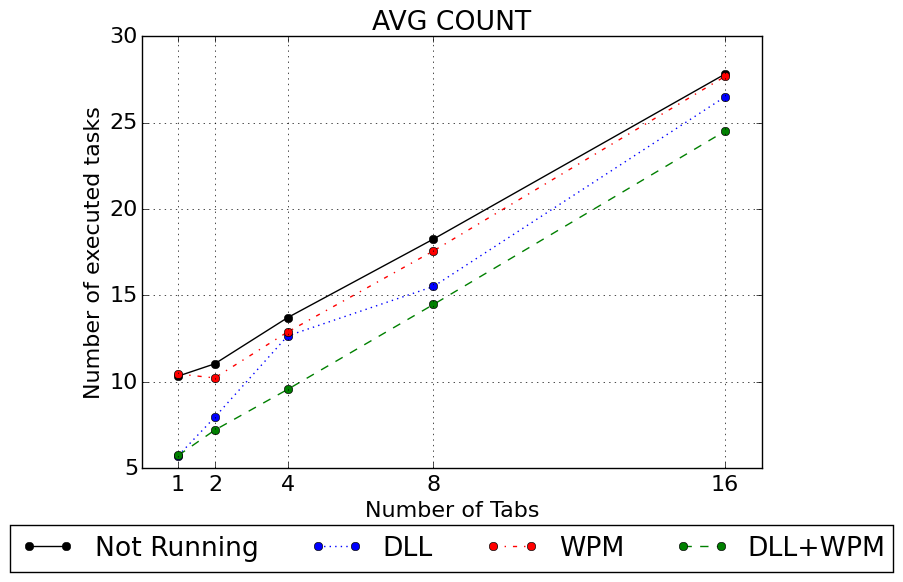
\includegraphics[width=\textwidth,height=0.45\textheight,keepaspectratio]{Evaluation/experiment1/AVG-COUNT-2.png}
    \caption{Average count, 2 minutes of data}
    \label{fig:ex1_avgcount_2}

  	\vspace*{\floatsep}
  	
    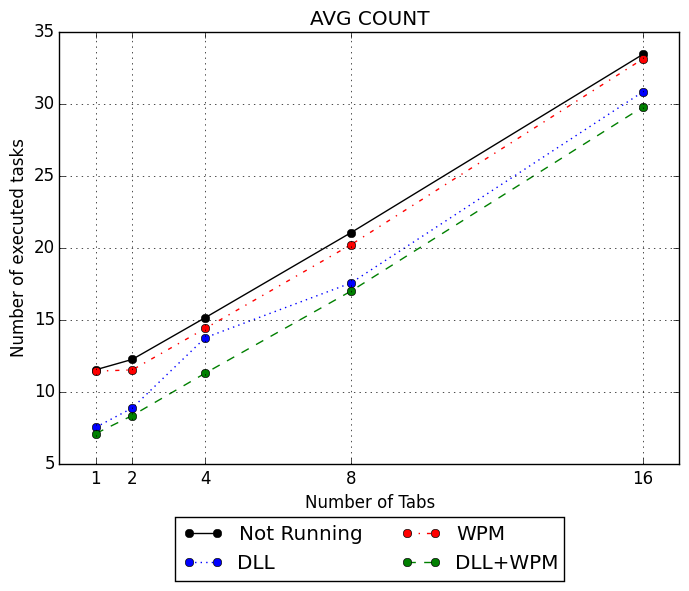
\includegraphics[width=\textwidth,height=0.45\textheight,keepaspectratio]{Evaluation/experiment1/AVG-COUNT-16.png}
    \caption{Average count, 16 minutes of data}
    \label{fig:ex1_avgcount_16}
\end{figure}
Figure \ref{fig:ex1_avgcount_2} shows the average count of tasks that were executed over two minutes. Running both components, \emph{\gls{DLL}+\gls{WPM}} is the slowest of all four configurations, because the average number of executed tasks is the lowest. \emph{WPM} and the \emph{Not Running} are almost equal with \emph{\gls{WPM}} being one task slower in for two and fours tabs. Figure \ref{fig:ex1_avgcount_16} shows the same measurement for a duration of 16 minutes. The result is the same as of Figure \ref{fig:ex1_avgcount_2}. The comparison between both plots show that there is not much of a difference between a one and 16 minute measurement, but the 16 minute measurements give more accurate results. What is more interesting about these graphs is the linear trend of the four plots. For each added tab only about 1.5 times more tasks are executed. This is consistent throughout all four plots.
\begin{figure}[!htbp]
	\centering
    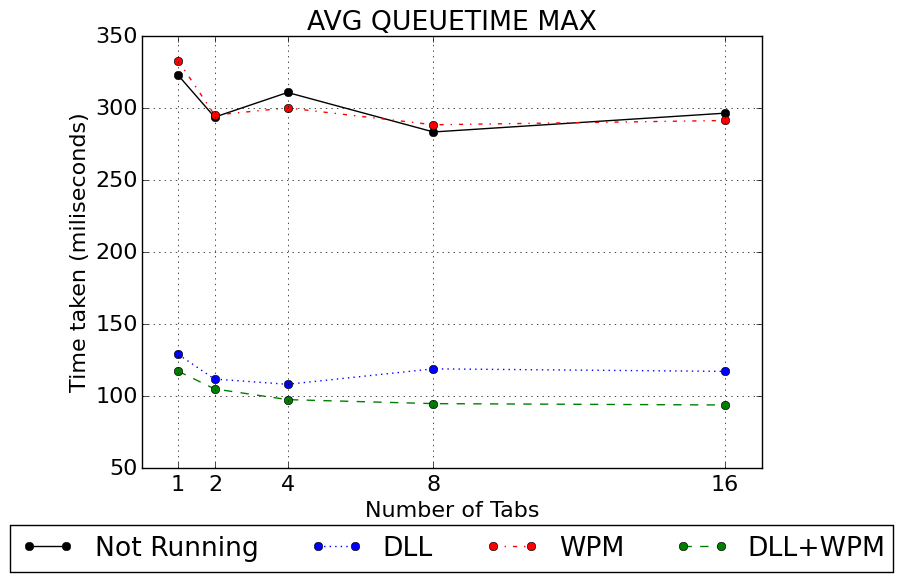
\includegraphics[width=\textwidth,height=0.45\textheight,keepaspectratio]{Evaluation/experiment1/AVG-QUEUETIME-MAX-1.png}
    \caption{Average of the maximum queuetime, 1 minute of data}
    \label{fig:ex1_avgqueuetimemax_1}

	\vspace*{\floatsep}

    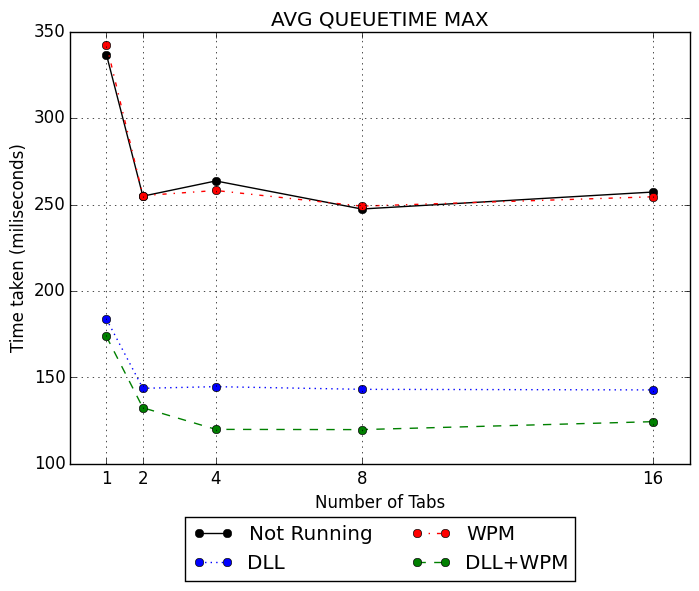
\includegraphics[width=\textwidth,height=0.45\textheight,keepaspectratio]{Evaluation/experiment1/AVG-QUEUETIME-MAX-16.png}
    \caption{Average of the maximum queuetime, 16 minutes of data}
    \label{fig:ex1_avgqueuetimemax_16}
\end{figure}
This property of Chrome being faster (executing more task) without a driver running can be seen too in the next two Figures \ref{fig:ex1_avgqueuetimemax_1} and \ref{fig:ex1_avgqueuetimemax_16}. These graphs show the average of the maximum queuetime. The y-axis shows the average number of milliseconds a task was waiting for execution. Again, two groups form, \emph{Not Running} with \emph{\gls{WPM}} and \emph{\gls{DLL}} and \emph{\gls{DLL}+\gls{WPM}}. Tasks without running driver queue in average longer than tasks with running driver. The reason for that is \emph{Not running} executes more tasks, which leads to some tasks queuing longer because Chrome is busy with running other tasks. Accordingly, the average queuetime for the \gls{DLL} component and both components running is lower, because less tasks are executed and Chrome is less busy with task execution. The overhead of the driver is clearly present in the figures and tasks are in average waiting 100 milliseconds less than without running the driver. This means, that the average overhead per task introduced to the driver is 100 milliseconds for the queuetime.
\begin{figure}[!htbp]
	\centering
    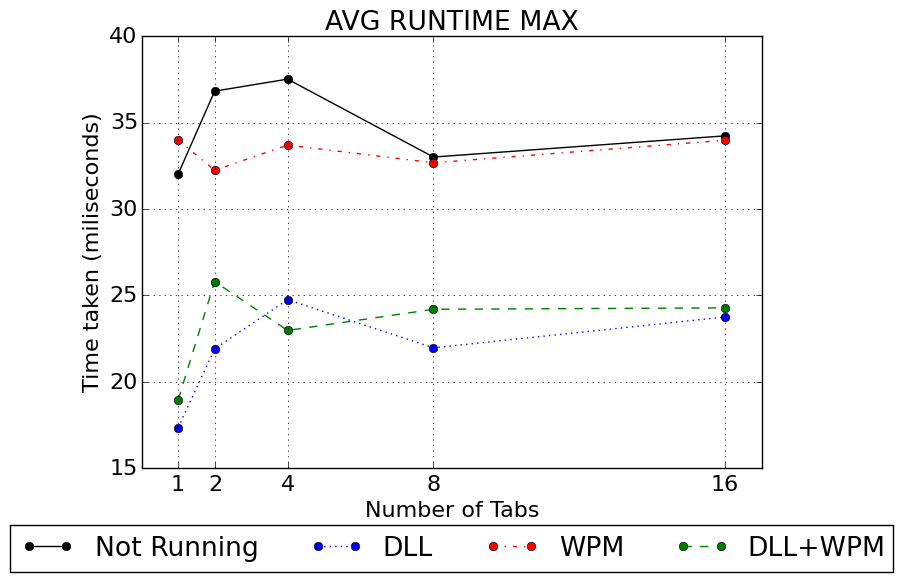
\includegraphics[width=\textwidth,height=0.45\textheight,keepaspectratio]{Evaluation/experiment1/AVG-RUNTIME-MAX-1.png}
    \caption{Average of the maximum runtime, 1 minute of data}
    \label{fig:ex1_avgruntimemax_1}
    
  	\vspace*{\floatsep}    
    
    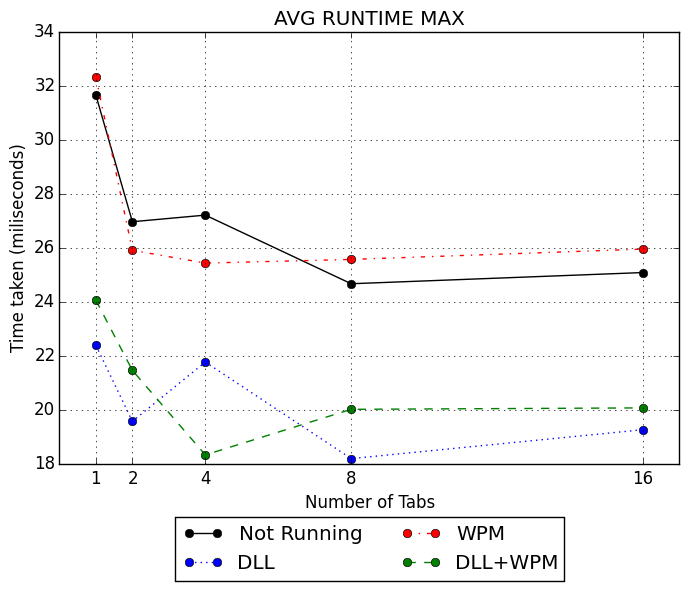
\includegraphics[width=\textwidth,height=0.45\textheight,keepaspectratio]{Evaluation/experiment1/AVG-RUNTIME-MAX-16.png}
    \caption{Average of the maximum runtime, 16 minutes of data}
    \label{fig:ex1_avgruntimemax_16}
\end{figure}
Figure \ref{fig:ex1_avgruntimemax_1} and Figure \ref{fig:ex1_avgruntimemax_16} show the average of the maximum runtime of all tasks for one and 16 minutes. The results of this plots are similar to Figure \ref{fig:ex1_avgqueuetimemax_1} and Figure \ref{fig:ex1_avgqueuetimemax_16}. The average runtime of \emph{Not Running} and \emph{\gls{WPM}} is higher than \emph{\gls{DLL}} and \emph{\gls{DLL}+\gls{WPM}}. This is again a result of the higher number of tasks executed and Chrome being already busy executing other tasks. Additionally, tasks are waiting for other tasks to be finished with execution, extending the runtime.
\begin{figure}[!htbp]
	\centering
    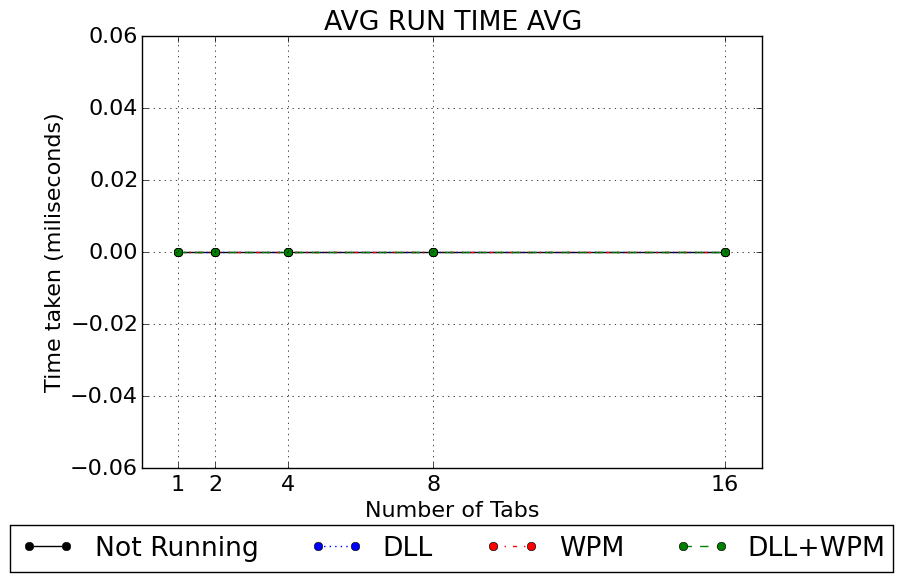
\includegraphics[width=\textwidth,height=0.45\textheight,keepaspectratio]{Evaluation/experiment1/AVG-RUNTIME-AVG-1.png}
    \caption{Average of the average runtime, 1 minute of data}
    \label{fig:ex1_avgruntimeavg_1}
    
  	\vspace*{\floatsep}    
    
    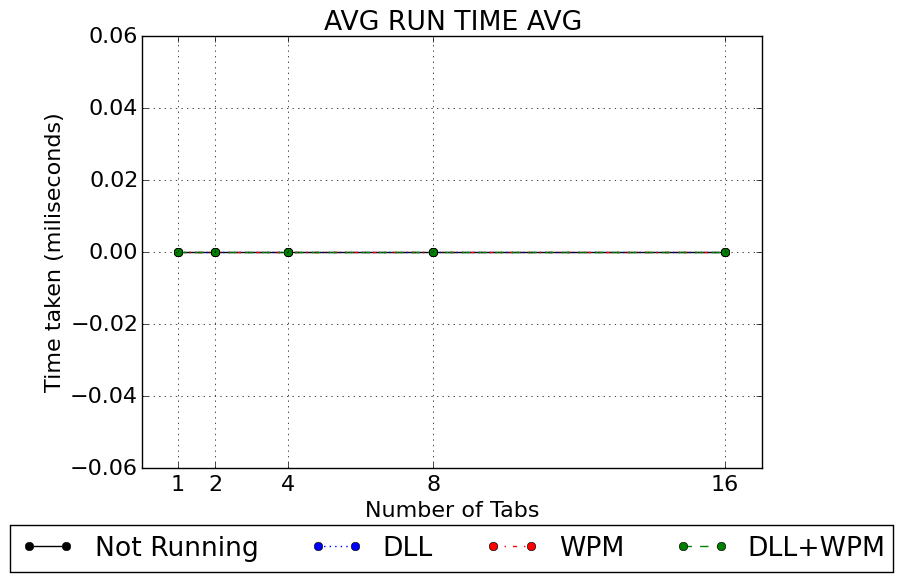
\includegraphics[width=\textwidth,height=0.45\textheight,keepaspectratio]{Evaluation/experiment1/AVG-RUNTIME-AVG-16.png}
    \caption{Average of the average runtime, 16 minutes of data}
    \label{fig:ex1_avgruntimeavg_16}
\end{figure}
At the end of this experiment, a look is taken at the average of the average runtime of a task. This data is shown in Figure \ref{fig:ex1_avgruntimeavg_1} for one minute and Figure \ref{fig:ex1_avgruntimeavg_16} for 16 minutes. The result is, that there is in average no difference between running the driver and not running it. For both Figures, the average runtimes are zero. This means, because the runtimes are using rounded values, the execution took less than 0.50 milliseconds in average.

\medskip

The result of this experiment 1 is, that the driver slows down execution during startup, which increase maximum run- and queuetime. There is no difference during the later usage, as the average of the average runtimes are staying constant. The reason for this performance decrease can be found in the \gls{DLL} component of the driver, as the other one, the \gls{WPM} component is running with almost no performance decrease. The \gls{DLL} component will be evaluated further in experiment 2.
\clearpage
\subsubsection{Experiment 2}
\begin{figure}[h]
	\centering
    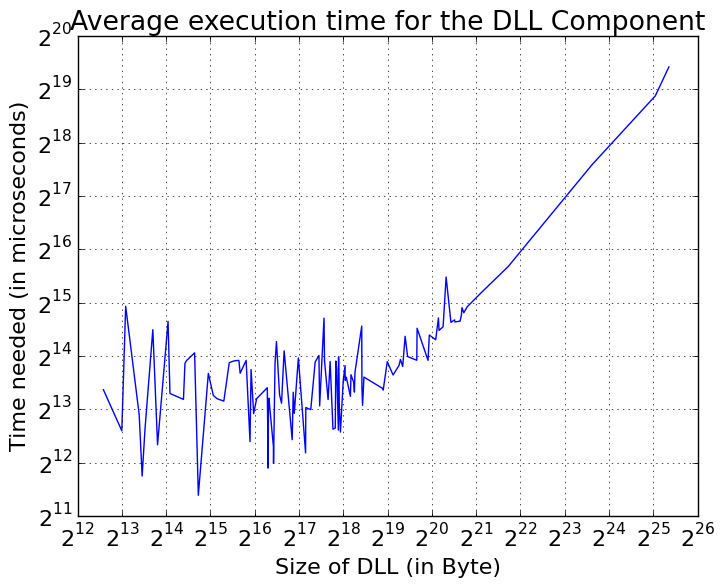
\includegraphics[width=\textwidth,height=0.45\textheight,keepaspectratio]{Evaluation/experiment2/result.png}
    \caption{Average execution time for sha256 file hashing}
    \label{fig:ex2_result}
\end{figure}
In Experiment 2 the performance impact of the \gls{DLL} component is evaluated. Experiment 2 uses the same hardware and software setup as Experiment 1. As the result of Experiment 1 showed, that running the \gls{DLL} component slowed down the execution of \emph{Google Chrome}, Experiment 2 tries to find the actual reason for that result. Looking at the code, and running time measurements on it leads to the sha256 file hashing slowing down the execution. Figure~\ref{fig:ex2_result} shows the average of ten independent measurements. For file sizes between four kilobyte ($2^{12}$ byte) and one megabyte ($2^{20}$ byte), the needed time is roughly constant around 16 milliseconds ($2^{14}$ microseconds). Increasing the file size further than one megabyte results into increase of time for hashing the file. The graph uses logarithmic scaling with base two one both axis, which give a better comparability of the actual result. Starting at one megabyte, doubling the file size will double the necessary time to create the sha256 hash. Most \glspl{DLL} are rather small (less than one megabyte) and will require constant time for file hashing. However, in contrast to that, some are very large (around 50 megabyte or even larger) and will require with respect to the given file size linearly more time. An example for that can be found in \emph{Google Chrome's} used \glspl{DLL}. \emph{Chrome\_child.dll} with 40 megabyte and \emph{chrome.dll} with 30 megabyte make up most of the time that is spent for hashing during \emph{Chrome's} process creation. As the initial callback function \syscall{PsSetLoadImageNotifyRoutine} is acting synchronous, so is the hashing of files. Therefore, the process is suspended for the whole time that is needed for hashing all \glspl{DLL}. A single process creation is delayed by the sum of the required time for hashing all \glspl{DLL}, which makes up a total of 2905253 microseconds, or 2.9 seconds.

\paragraph{Impact of \gls{DLL} injections}
In case of an actual attack with \gls{DLL} injections, it is interesting to know which performance impact is present for \emph{Google Chrome}. According to Experiment 2, the time required for hashing is
\begin{equation}
t(x) = \min\{2^{14} * 2^{\log_2(x) - 20}, 2^{14}\} \label{eq:one}
\end{equation}
where $x$ is the file size in bytes of the \gls{DLL} and $t(x)$ is the required time in microseconds for calculating the hash. The time cost of (\ref{eq:one}) is scaling linearly with the size $x$ of the \gls{DLL} file. Therefore, especially for larger files it is interesting to know if hashing is required every time the \gls{DLL} is mapped into memory. In the current implementation, hashing occurs only once, if the \gls{DLL} is not on the whitelist. This is due to \emph{Windows} internal \gls{DLL} loading behavior. The result of patching a \gls{DLL} is an invalid executable format. As soon as a second \gls{DLL} load request for the same file is done, the \emph{Windows} kernel will return early with error \syscall{ERROR\_BAD\_EXE\_FORMAT}. This behavior will stay until the file is unloaded from memory which will happen when exiting \emph{Chrome}. In the other case, where the \gls{DLL} is in the whitelist, there is no such way of returning early. The \gls{DLL} file will need to be hashed again if it is not present in the process virtual memory. This is another limitation of the approach using \syscall{PsSetLoadImageNotifyRoutine}.
\subsection{Security}
\section{Conclusion and Future work}
\label{sec:futurework}
This chapter summarizes the thesis, draws a conclusion and includes the limitations of the proposed solution. After that an outline is given for potential future work.
\subsection{Summary}
The thesis has introduced a kernelmode driver to tackle the problem of \gls{PMT}. The different kinds of attacks have been grouped into two categories, external and internal modifications. As such, they were handled separately when designing the architecture of the proposed solution. \gls{WPM} and \gls{DLL} component have been introduced to handle the respective memory tampering and \gls{DLL} injection attacks. Section~\ref{sec:performance}~and~\ref{sec:security} analyzed the performance and security of the proposed solution. While the \gls{WPM} component resulted in almost no overhead, running the \gls{DLL} component resulted in a huge performance hit. During execution of the \gls{DLL} component, the process gets suspended for the time a hash is generated. It was found out, that the required time scales exponentially with the file size. The performance overhead is therefore the first limitation of the proposed solution. Security analysis outlined that the attacker can not bypass the driver from restricting his actions, given certain conditions. The first condition is that the privilege level of the attacker may not be higher than user privileges (i.e., no admin privileges). The second condition is, that identification of the process which should receive \gls{PMT} protection must be ensured (i.e., the attacker is not allowed to rename the process executable file name). All three limitations can possibly be solved by further research in this area.
\subsection{Future work}
This section will give an outline about possible future research involving this thesis and \gls{PMT}.
\subsubsection{DLL hash caching}
The proposed solution has a performance overhead during \gls{DLL} hashing. This is because every \gls{DLL} might get hashed multiple times, despite no actual changes to the file. In some cases, the \gls{DLL} might also get hashed multiple times for the same process. Future research could develop a method to cache the generated \gls{DLL} hash. The overhead of the \gls{DLL} component will get significantly reduced, making hashing a one time cost until file changes are recognized. 
\subsubsection{Process identification}
Identification of a process is not easily possible in the current solution. The proposed solution uses the executable's file name which can be changed by the attacker. Even generating a hash over this file will not be enough to identify the process that should receive \gls{PMT} protection. Future research could develop a method to identify a process based on a stronger heuristic than file name or file hash. This will make the proposed solution harder to bypass.
\subsubsection{Driver extension to other processes}
The proposed solution currently only works for \emph{Google Chrome}. The driver uses hard coded values to identify a \emph{Chrome} process and will not work on other processes without further extension. Future research could develop a method to apply \gls{PMT} protection to other processes by introducing a standardized specification that allows to protect multiple independent processes. The specification outcome could then be deployed by the application vendors to make use of the installed driver. The implementation must ensure, that the introduced specification will not compromise the drivers security.
\subsubsection{Driver to process communication}
Updating of an application like \emph{Google Chrome} is currently not possible because the proposed solution uses a hard coded whitelist. A dynamic whitelist would be beneficial but will require communication between the driver and the application. Future research could develop a method for safe communication between driver and application. This will allow on-the-fly updating of applications. Communication between driver and application will thus reduce the number of \glspl{DLL} that need to be hashed.

\section{Chrome ELF DLL}
Google Chrome contains a built in chrome\_elf.dll file that serves various important and security relevant functions. The main three functionalities are export of functions, caching of function addresses of important DLL files and a built in DLL blacklist. Chrome ELF is the very first loaded module in Chrome and could be used to imply more security features like setting a process security descriptor\footnote{This concept is evaluated later in chapter \ref{sec:implementation_dacl}}, however - as Google's development team states - they aren't interested in protecting Chrome from user-mode injection\cite{chromium_security}. This is due to the reason, that a malicious process running under the same process could employ any modification that cannot be prevented by Chrome itself. The user should rely on his installed anti-virus software to detect and prevent attacks.
\subsection{Exported Functions}
 
\subsection{Cached function addresses}
The second part of Chrome ELFs features is a built in caching of function addresses of ntdll.dll. All exported functions are stored inside a function lookup table to increase speed and reduce lookup operations of this often used functions. Additionally, the virtual memory space of the function lookup table is set to PAGE\_READONLY, to ensure that this memory can no longer be modified. Again, this adds no security as an attacker (from in or outside) will simply undo this operation and modify the lookup table. Additionally, this feature creates a whole new threat that can be easily used for attacks. Entries of the lookup table receive a new address, making the more complicated API Hooking attacks unneccessary.
\subsection{DLL Blacklist}
Chrome ELF contains a DLL blacklist feature, which automatically prevents unwanted DLLs from being run inside Chrome. The blacklist is split into two parts, the first contained inside the code and a second list loaded from the local computers registry. The existing detection algorithms checks for an existing entry in the blacklist by comparing the file- and imagename of the loaded DLL file. If a blacklisted DLL is found, [........] unloads the DLL from Chrome and ensures that it is no longer contained inside the process' virtual memory. However, this algorithms adds no security! A comparison between file-/imagenames is very weak, as an attacker might simply change the name of the DLL file. Additionally, every new build of the blacklisted module will not be detected if the name is changed. The whole purpose of the existing blacklist feature is to increase stability of Google Chrome and prevent instable extensions and addons from running, to ensure an as optimal as possible user experience inside the browser.
 
% References
\section{References}
\bibliography{references}
\bibliographystyle{plain}
% PUT Appendix here!
\section{Appendix A}
\label{sec:appendix}

\subsection{Example DLL Injection with SetWindowsHookEx}
The following code shows a DLL injection using the SetWindowsHookEx function.

\subsection{Example DLL Injection with WriteProcessMemory}
The following code shows a DLL injection using the WriteProcessMemory function.

\subsection{DACL Testing Application}
The following shows the minimum required code for setting a DACL to prevent WriteProcessMemory calls.
\codefile{ProcessDACL/ProcessDACL/}{processDacl.cpp}

\subsection{Driver Program}

In the following sections, the result of the Design and Implementation task, a driver is shown, created in the C programming language.
\codefile{main.c}
\codefile{common.h}
\codefile{stdafx.h}
\codefile{image_load_routine.h}
\codefile{image_load_routine.c}
\codefile{memory.h}
\codefile{memory.c}
\codefile{obcallback_routine.h} 
\codefile{obcallback_routine.c}
\codefile{proc_create_routine.h} 
\codefile{proc_create_routine.c}
\codefile{ptree.h} 
\codefile{ptree.c} 
\codefile{sha2.h} 
\codefile{sha2.c} 
\codefile{whitelist.h} 
\codefile{whitelist.c} 


\end{document}
